
\subsection{Gini-based optimization strategies}\label{S:GINI}


\subsubsection{Gini dispersion measure}
As we mentioned, \GINI\ dispersion measure is given by Eq.~(\ref{hmod2}) for $p=1$, \ie,
\begin{equation}
    \GINI = \frac{1}{N^2}\sum_{i=1}^{N-1}\sum_{j=i+1}^N \left| r_i - r_j \right|,
    \label{gini0}
\end{equation}
where $r_i$ is the rate of return $i$-th historical observation.

Numerically, \GINI\ measure can be evaluated directly using Eq.~(\ref{gini0}). However, the computation can be
speed up significantly by transforming the double sum in a single sum.

Let $\{x_i\}_{i=1,\cdots,N}$ be $\{r_i\}_{i=1,\cdots,N}$ sorted in ascending order. Then, after some straightforward
algebraic manipulations, Eq.~(\ref{gini0}) can be rewritten as
\begin{equation}
    \GINI = \frac{1}{N^2}\sum_{i=1}^N (2 i - N  + 1) x_i.
    \label{gini00}
\end{equation}
A computation algorithm based on
Eq.~(\ref{gini00}), assuming a heapsort algorithm followed by a single sum, has a complexity of $\cO(N \log(N))$,
while an algorithm based on Eq.~(\ref{gini0}), involving a double sum, has a complexity of $\cO(N^2)$, where $N$ is
the number of observations.\footnote{As a guideline, a typical value for $N$ is $1,000$.}
Therefore, the evaluation of \GINI\ based on Eq.~(\ref{gini00}) is faster.
This approach has been implemented in the \azapy\ package.

\BackToContents

\subsubsection{Gini optimal portfolio}
This optimization is described by Eqs.~(\ref{gg1}) from Sec~\ref{strategies} point~\ref{OptRisk},
where $\rho$ is given by \GINI\ from Eq.\ (\ref{gini0}).
It is the following LP problem.

\bigskip
\noindent Minimize over $\{ \{w_k\}_{k=1,\cdots,M}, \{s_{ij}\}_{i=1,\cdots,N-1; j = i+1,\cdots,N} \}$
\begin{subequations}\label{gini1}
\begin{align}
    &g = \frac{1}{N^2} \sum_{i=1}^{N-1} \sum_{j = i+1}^N s_{ij}, \label{gini1a} \\
    \st &s_{ij} \geq \sum_{k=1}^M w_k (r_{ki} - r_{kj}), \label{gini1b} \\
        &s_{ij} \geq -\sum_{k=1}^M w_k (r_{ki} - r_{kj}), \label{gini1c} \\
        &\sum_{k=1}^M w_k \mu_k \geq \mu, \label{gini1d} \\
        & \sum_{k=1}^M w_k = 1, \label{gini1e} \\
        & s_{ij} \geq 0, \label{gini1g} \\
        & w_k \geq 0, \label{gini1f}
\end{align}
\end{subequations}

\noindent where $\mu$ in Eq.~(\ref{gini1d}) is the portfolio targeted rate of return while $\{\mu_k\}_{i=1,\cdots,M}$
are the portfolio components expected rate of returns.
Then, we have
\begin{subequations}\label{gini2}
\begin{align}
    \RR &= \sum_{k=1}^M w_k^* \mu_k, \label{gini2a} \\
    \GINI &= g^*, \label{gini2b}
\end{align}
\end{subequations}

\noindent where $^*$ denotes the solution of LP problem.
In addition to the portfolio weights $\{w_k^*\}_{k=1,\cdots,M}$ and expected rate of return $\RR$, the
LP solution provides information about the portfolio \GINI\ dispersion.

The number of variables in the LP from Eqs.\ (\ref{gini1}) is $M + N(N-1)/2$. It scales quadratic with the number
of historical observations, $N$.
This rapid grow of dimensionality, leading to excessive computational efforts, is the main disadvantage of any \GINI-based optimal portfolio
strategy evaluation. However, keeping the length of historical observation at reasonable values (say, 1-2 year) the \GINI-based
optimization strategies are numerically tractable.

\bigskip
\noindent Here is an example, using the \azapy\ package, of how to compute the \GINI\ optimal portfolio.
The \GINI\ time horizon was set to one quarter and the calibration is performed using 1.25 years of
close-adjusted historical prices (default settings).
For more details see the package documentation at \azapydoc.

\lstinputlisting[language=Python]{../PyScripts/Gini_RiskOptim.py}

\BackToContents


\subsubsection{Minimum Gini portfolio}

Following the results from Sec.~\ref{strategies} point~\ref{MinRisk},
the algorithm to compute the optimal portfolio with minimum \GINI\ dispersion is given by the LP problem from Eqs.~(\ref{gini1}) where
$\mu$ from r.h.s. of Eq.~(\ref{gini1d}) is set to a value equal to the smallest expected rate of
return among the portfolio components, \ie\ $\mu=\min_k\{\mu_k\}$.

\bigskip
\noindent Here is an example, using the \azapy\ package, of how to compute the minimum \GINI\ portfolio.
The \GINI\ time horizon was set to one quarter and the calibration is performed using 1.25 years of
close-adjusted historical prices (default settings).
For more details see the package documentation at \azapydoc.

\lstinputlisting[language=Python]{../PyScripts/Gini_MinRisk.py}

\BackToContents


\subsubsection{Gini optimal portfolio for targeted risk value}
This optimization is described by  Eqs.~(\ref{gg2}) from Sec~\ref{strategies} point~\ref{MinRisk},
where $\rho$ is given by \GINI\ from Eq.~(\ref{gini0}).
It is the following LP problem.

\bigskip
\noindent Maximize over $\{ \{w_k\}_{k=1,\cdots,M}, \{s_{ij}\}_{i=1,\cdots,N-1; j = i+1,\cdots,N} \}$
\begin{subequations}\label{gini3}
\begin{align}
    &g = \sum_{k=1}^M w_k \mu_k , \label{gini3a} \\
    \st & \frac{1}{N^2} \sum_{i=1}^{N-1} \sum_{j = i+1}^N s_{ij} = \GINI_0, \label{gini3d} \\
        & s_{ij} \geq \sum_{k=1}^M w_k (r_{ki} - r_{kj}), \label{gini3b} \\
        & s_{ij} \geq -\sum_{k=1}^M w_k (r_{ki} - r_{kj}), \label{gin3c} \\
        & \sum_{k=1}^M w_k = 1, \label{gini3e} \\
        & s_{ij} \geq 0, \label{gini3g} \\
        & w_k \geq 0, \label{gin3f}
\end{align}
\end{subequations}

\noindent where $\GINI_0$ from Eq.~(\ref{gini3d}) is the targeted portfolio \GINI\ dispersion value.
Then, the portfolio expected rate of return is given by the value of the objective
function, \ie,
\begin{equation}
    \RR = g^*, \label{gini4}
\end{equation}

\noindent and the optimal portfolio weights by $\{w^*_k\}_{k=1,\cdots,M}$. The superscript $^*$ denotes the
solution of LP problem.

\bigskip
\noindent Here is an example, using the \azapy\ package, of how to compute the optimal portfolio
with the same \GINI\ as the equal weighted portfolio.
The \GINI\ time horizon was set to one quarter and the calibration is performed using 1.25 years of
close-adjusted historical prices (default settings).
For more details see the package documentation at \azapydoc.

\lstinputlisting[language=Python]{../PyScripts/Gini_InvNrisk.py}

\BackToContents


\subsubsection{Gini optimal portfolio for fixed risk-aversion factor}
This optimization is described by Eqs.\ (\ref{gg3}) from Sec~\ref{strategies} point~\ref{MinRisk},
where $\rho$ is given by \GINI\ from Eq.\ (\ref{gini0}).
It is the following LP problem.

\bigskip
\noindent Maximize over $\{ \{w_k\}_{k=1,\cdots,M}, \{s_{ij}\}_{i=1,\cdots,N-1; j = i+1,\cdots,N} \}$
\begin{subequations}\label{gini5}
\begin{align}
    &g = \sum_{k=1}^M w_k \mu_k - \frac{\lambda}{N^2} \sum_{i=1}^{N-1} \sum_{j = i+1}^N s_{ij}, \label{gini5a} \\
    \st &s_{ij} \geq \sum_{k=1}^M w_k (r_{ki} - r_{kj}), \label{gini5b} \\
        &s_{ij} \geq -\sum_{k=1}^M w_k (r_{ki} - r_{kj}), \label{gini5c} \\
        & \sum_{k=1}^M w_k = 1, \label{gini5d} \\
        & s_{ij} \geq 0, \label{gini5f} \\
        & w_k \geq 0, \label{gini5e}
\end{align}
\end{subequations}

\noindent where $\lambda$ in Eq.\ (\ref{gini5a}) is the risk aversion coefficients.
Then, we have
\begin{subequations}\label{gini6}
\begin{align}
    \RR &= \sum_{k=1}^M w_k^* \mu_k, \label{gini6a} \\
    \GINI &= \frac{\RR - g^*}{\lambda}, \label{gini6b}
\end{align}
\end{subequations}

\noindent where $^*$ denotes the solution of LP problem.
In addition to the portfolio weights $\{w_k^*\}_{k=1,\cdots,M}$, the
LP solution provides information about the portfolio \GINI\ dispersion.

\bigskip
\noindent Here is an example, using the \azapy\ package, of how to compute the optimal portfolio
for a given value of the risk aversion coefficient $\lambda$.
The \GINI\ time horizon was set to one quarter and the calibration is performed using 1.25 years of
close-adjusted historical prices (default settings).
For more details see the package documentation at \azapydoc.

\lstinputlisting[language=Python]{../PyScripts/Gini_Averse.py}

\BackToContents


\subsubsection{Gini-Sharpe optimal portfolio - maximization solution}
This optimization targets the maximization of \GINI-Sharpe ratio. It is based on the
Eqs.~(\ref{gg4}) from Sec~\ref{strategies} point~\ref{MinRisk},
where $\rho$ is given by \GINI\ from Eq.~(\ref{gini0}).
The optimization can be formulated as an LP problem
if Eq.~(\ref{gg4b}) can be linearized. In our case the linearization is straightforward. Introducing the
variable transformations $\bw_k = t w_k$ and $\bs_{li} = t s_{li}$, the LP
problem can be written as follows.

\bigskip
\noindent Maximize over $\{ \{\bw_k\}_{k=1,\cdots,M}, \{\bs_{ij}\}_{i=1,\cdots,N-1; j = i+1,\cdots,N}, t \}$
\begin{subequations}\label{gini7}
\begin{align}
    &g = \sum_{k=1}^M \bw_k \mu_k - \mu_0 t, \label{gini7a} \\
    \st &\frac{1}{N^2} \sum_{i=1}^{N-1} \sum_{j=i+1}^N \bs_{ij} = 1, \label{gini7d} \\
        &\bs_{ij} \geq \sum_{k=1}^M \bw_k (r_{ki} - r_{kj}), \label{gini7b} \\
        &\bs_{ij} \geq -\sum_{k=1}^M \bw_k (r_{ki} - r_{kj}), \label{gini7c} \\
        & \sum_{k=1}^M \bw_k - t = 0, \label{gini7e} \\
        & t \geq 0, \label{gini7h} \\
        & \bs_{ij} \geq 0, \label{gini7g} \\
        & \bw_k \geq 0, \label{gini7f}
\end{align}
\end{subequations}


\noindent where $\mu_0$ in Eq.~(\ref{gini7a}) is the
risk-free rate accessible to the investor.
Then, we have
\begin{subequations}\label{gini8}
\begin{align}
    w_k &= \frac{\bw_k^*}{t^*} , \label{gini8a} \\
    \RR &= \frac{g^*}{t^*} + \mu_0, \label{gini8c} \\
    \Sharpe &= g^*, \label{gini8b} \\
    \GINI &= \frac{1}{t^*}, \label{gini8d}
\end{align}
\end{subequations}

\noindent where $^*$ denotes the solution of LP problem.
In addition to the optimal portfolio weights $\{w_k\}_{k=1,\cdots,M}$, expected rate of return $\RR$ and
\GINI-Sharpe ratio $\Sharpe$,
the LP solution provides information about the portfolio \GINI\ dispersion.

\bigskip
\noindent Here is an example, using the \azapy\ package, of how to compute the \GINI-Sharpe optimal portfolio using the maximization
of \GINI-Sharpe ratio.
The \GINI\ time horizon was set to one quarter and the calibration is performed using 1.25 years of
close-adjusted historical prices (default settings).
For more details see the package documentation at \azapydoc.

\lstinputlisting[language=Python]{../PyScripts/Gini_Sharpe.py}

\BackToContents


\subsubsection{Gini-Sharpe optimal portfolio - minimization solution}
This optimization targets the minimization of the inverse of \GINI-Sharpe ratio.
It is  described by Eqs.~(\ref{gg8}) from Sec.~\ref{strategies} point~\ref{MinSharpe}, where
$\rho$ is given by \GINI\ from Eq.~(\ref{gini0}).
The optimization can be formulated as an LP problem if Eq.~(\ref{gg8a}) can be linearized. This can be achieved by
introducing the variable transformations
$\bw_k = t w_k$ and $\bs_{li} = t s_{li}$.
Then, the LP problem can be written as follows.

\bigskip
\noindent Minimize over $\{ \{\bw_k\}_{k=1,\cdots,M}, \{\bs_{ij}\}_{i=1,\cdots,N-1; j = i+1,\cdots,N}, t \}$
\begin{subequations}\label{gini9}
\begin{align}
    &g = \frac{1}{N^2} \sum_{i=1}^{N-1} \sum_{j=i+1}^N \bs_{ij}, \label{gini9a} \\
    \st & \sum_{k=1}^M \bw_k\mu_k - \mu_0 t = 1, \label{gini9d} \\
        &\bs_{ij} \geq \sum_{k=1}^M \bw_k (r_{ki} - r_{kj}), \label{gini9b} \\
        &\bs_{ij} \geq -\sum_{k=1}^M \bw_k (r_{ki} - r_{kj}), \label{gini9c} \\
        & \sum_{k=1}^M \bw_k - t = 0, \label{gini9e} \\
        & t \geq 0, \label{gini9g} \\
        & \bs_{ij} \geq 0, \label{gini9h} \\
        & \bw_k \geq 0, \label{gini9f}
\end{align}
\end{subequations}

\noindent where $\mu_0$ in Eq.~(\ref{gini9d}) is the risk-free rate accessible to the investor.
Then we have,
\begin{subequations}\label{gini10}
\begin{align}
    w_k &= \frac{\bw_k^*}{t^*} , \label{gini10a} \\
    \RR &= \frac{1}{t^*} + \mu_0, \label{gini10c} \\
    \Sharpe &= \frac{1}{g^*}, \label{gini10b} \\
    \GINI &= \frac{g^*}{t^*}, \label{gini10d}
\end{align}
\end{subequations}

\noindent where $^*$ denotes the solution of LP problem.
In addition to the optimal portfolio weights $\{w_k\}_{k=1,\cdots,M}$, expected rate of return $\RR$ and
\GINI-Sharpe ratio $\Sharpe$,
the LP solution provides information about the portfolio \GINI\ dispersion.


\bigskip
\noindent Here is an example, using the \azapy\ package, of how to compute the \GINI-Sharpe optimal portfolio using the minimization
of the inverse of \GINI-Sharpe ratio.
The \GINI\ time horizon was set to one quarter and the calibration is performed using 1.25 years of
close-adjusted historical prices (default settings).
For more details see the package documentation at \azapydoc.

\lstinputlisting[language=Python]{../PyScripts/Gini_InvSharpe.py}

\BackToContents


\subsubsection{Gini frontiers}

Here is an example of how to compute the \GINI\ frontiers using the \azapy\
package. The \GINI\ time horizon was set to one quarter and the calibration is performed using 1.25 years of
close-adjusted historical prices (default settings).
For more details see the package documentation at \azapydoc.

The script produces the plots in Figs. \ref{GINI_fig1a} and \ref{GINI_fig1b}
for historical data collected up to 2021-07-27.

\lstinputlisting[language=Python]{../PyScripts/Gini_frontiers.py}

\begin{figure}[H]
\centering
\begin{subfigure}{.5\textwidth}
  \centering
  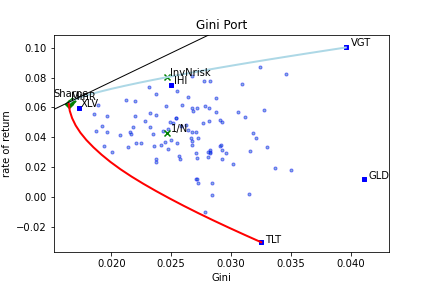
\includegraphics[width=.95\linewidth]{../figs/GINIFrontier1.png}
  \caption{Rate of return vs. \GINI}
  \label{GINI_fig1a}
\end{subfigure}%
\begin{subfigure}{.5\textwidth}
  \centering
  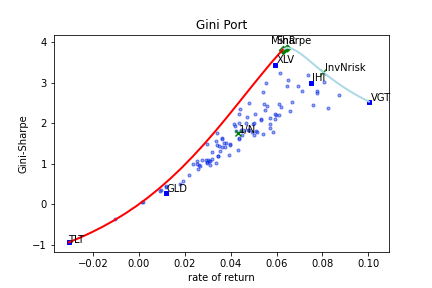
\includegraphics[width=.95\linewidth]{../figs/GINIFrontier2.png}
  \caption{\GINI-Sharpe vs. rate of return}
  \label{GINI_fig1b}
\end{subfigure}
\caption{\GINI\ frontiers.}
\label{GINI_fig1}
\end{figure}

\BackToContents

\subsubsection{Backtesting Gini-Sharpe optimal portfolio}

Here is an example, using \azapy\ package, of computing a portfolio backtesting.
For this example, we have chosen a portfolio quarterly rebalanced according
to the maximization of \GINI-Sharpe ratio. At each rebalancing date,
the portfolio weights
are calibrated based on 1.25 years of prior historical market data.

Other rebalancing strategies can be considered
by changing the value of {\it rtype} parameter in the call of {\it set\_model} function below.
For more details see the package documentation at \azapydoc.

\lstinputlisting[language=Python]{../PyScripts/Gini_Port.py}

\begin{figure}[H]
    \centering
    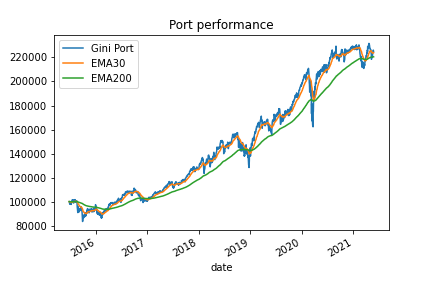
\includegraphics[width=.95\linewidth]{../figs/Port_GINI_Sharpe.png}
    \caption{Backtesting of quarterly rebalanced \GINI-Sharpe optimal portfolio.}
    \label{GINI_Port_fig}
\end{figure}

\BackToContents


